%KerMLSemanticsOverview.tex

\pn The Kernel Modeling Language (KerML) \cite{KerML} is intended to provide a foundation for more specific modeling languages.  SysML extends concepts in KerML for systems engineering.
 However, these supplemental semantics presume that KerML is being used for the purpose of systems engineering.

\pn For convenience, the applicable clause in the KerML specification is noted.  Some of its text is quoted without attribution or marking.

\section{Semantics (KerML 8.4)}

\comment{Some of the Semantics Overview is copied verbatim; some is rewritten for these semantics; stuff like OCL constraints is not mentioned at all, for now.}

\section{Semantics Overview (KerML 8.4.1)}

\pn A KerML model is intended to \bemph{represent} a system being modeled. The model is \bemph{interpreted} to make statements about the modeled system. The model may describe an existing system, in which case, if the model is correct, the statements it is interpreted to make about the system should all be true. A model may also be used to specify an imagined or planned system, in which case the statements the model is interpreted to make should be true for any system that is properly constructed and operated according to the model.

\pn Although a KerML model may represent a static system (like a bridge), most KerML models will \bemph{operate} necessitating different interpretations of model elements at different times.  For this, a \bemph{modal} logic is introduced in \S\ref{sec:modallogic}
%subclause 8.4.3.1.2 
and elaborated in Appendix \ref{chapter:KL}. % subclause 8.4.4.1.  
The modal logic defines \bemph{worlds} for different times during operation and an \bemph{interpretation} of model elements in each world.  Execution constructs an \bemph{execution model} $\mathfrak{M}$ either theoretically, or actual operation of the system.  To distinguish from an execution model, the KerML model humans create is often called a \bemph{design}.

\pn The \bemph{semantics} of KerML specify how a KerML model is to be interpreted. The semantics are defined in terms of the abstract syntax representation of the model, and only for models which are valid relative to the structure and constraints specified for the KerML abstract syntax. 
%As further specified in this subclause, m
Models expressed in KerML are given semantics by implicitly or explicitly using elements from  the Kernel Model Library. 
%These library models represent conditions on the structure and behavior of the system being modeled, which are further augmented in a user model as appropriate.

\pn A\comment{n understandable} formal specification of semantics allows models to be interpreted consistently. In particular, all KerML models extend library models expressed in KerML itself, understandable by KerML modelers. 
%These library models can then be ultimately reduced to a small, core subset of KerML, which is grounded in modal logic. 
The goal is to provide uniform model interpretation, which improves communication between everyone involved in modeling, including modelers and tool builders.

\begin{figure}[htbp]
\begin{center}
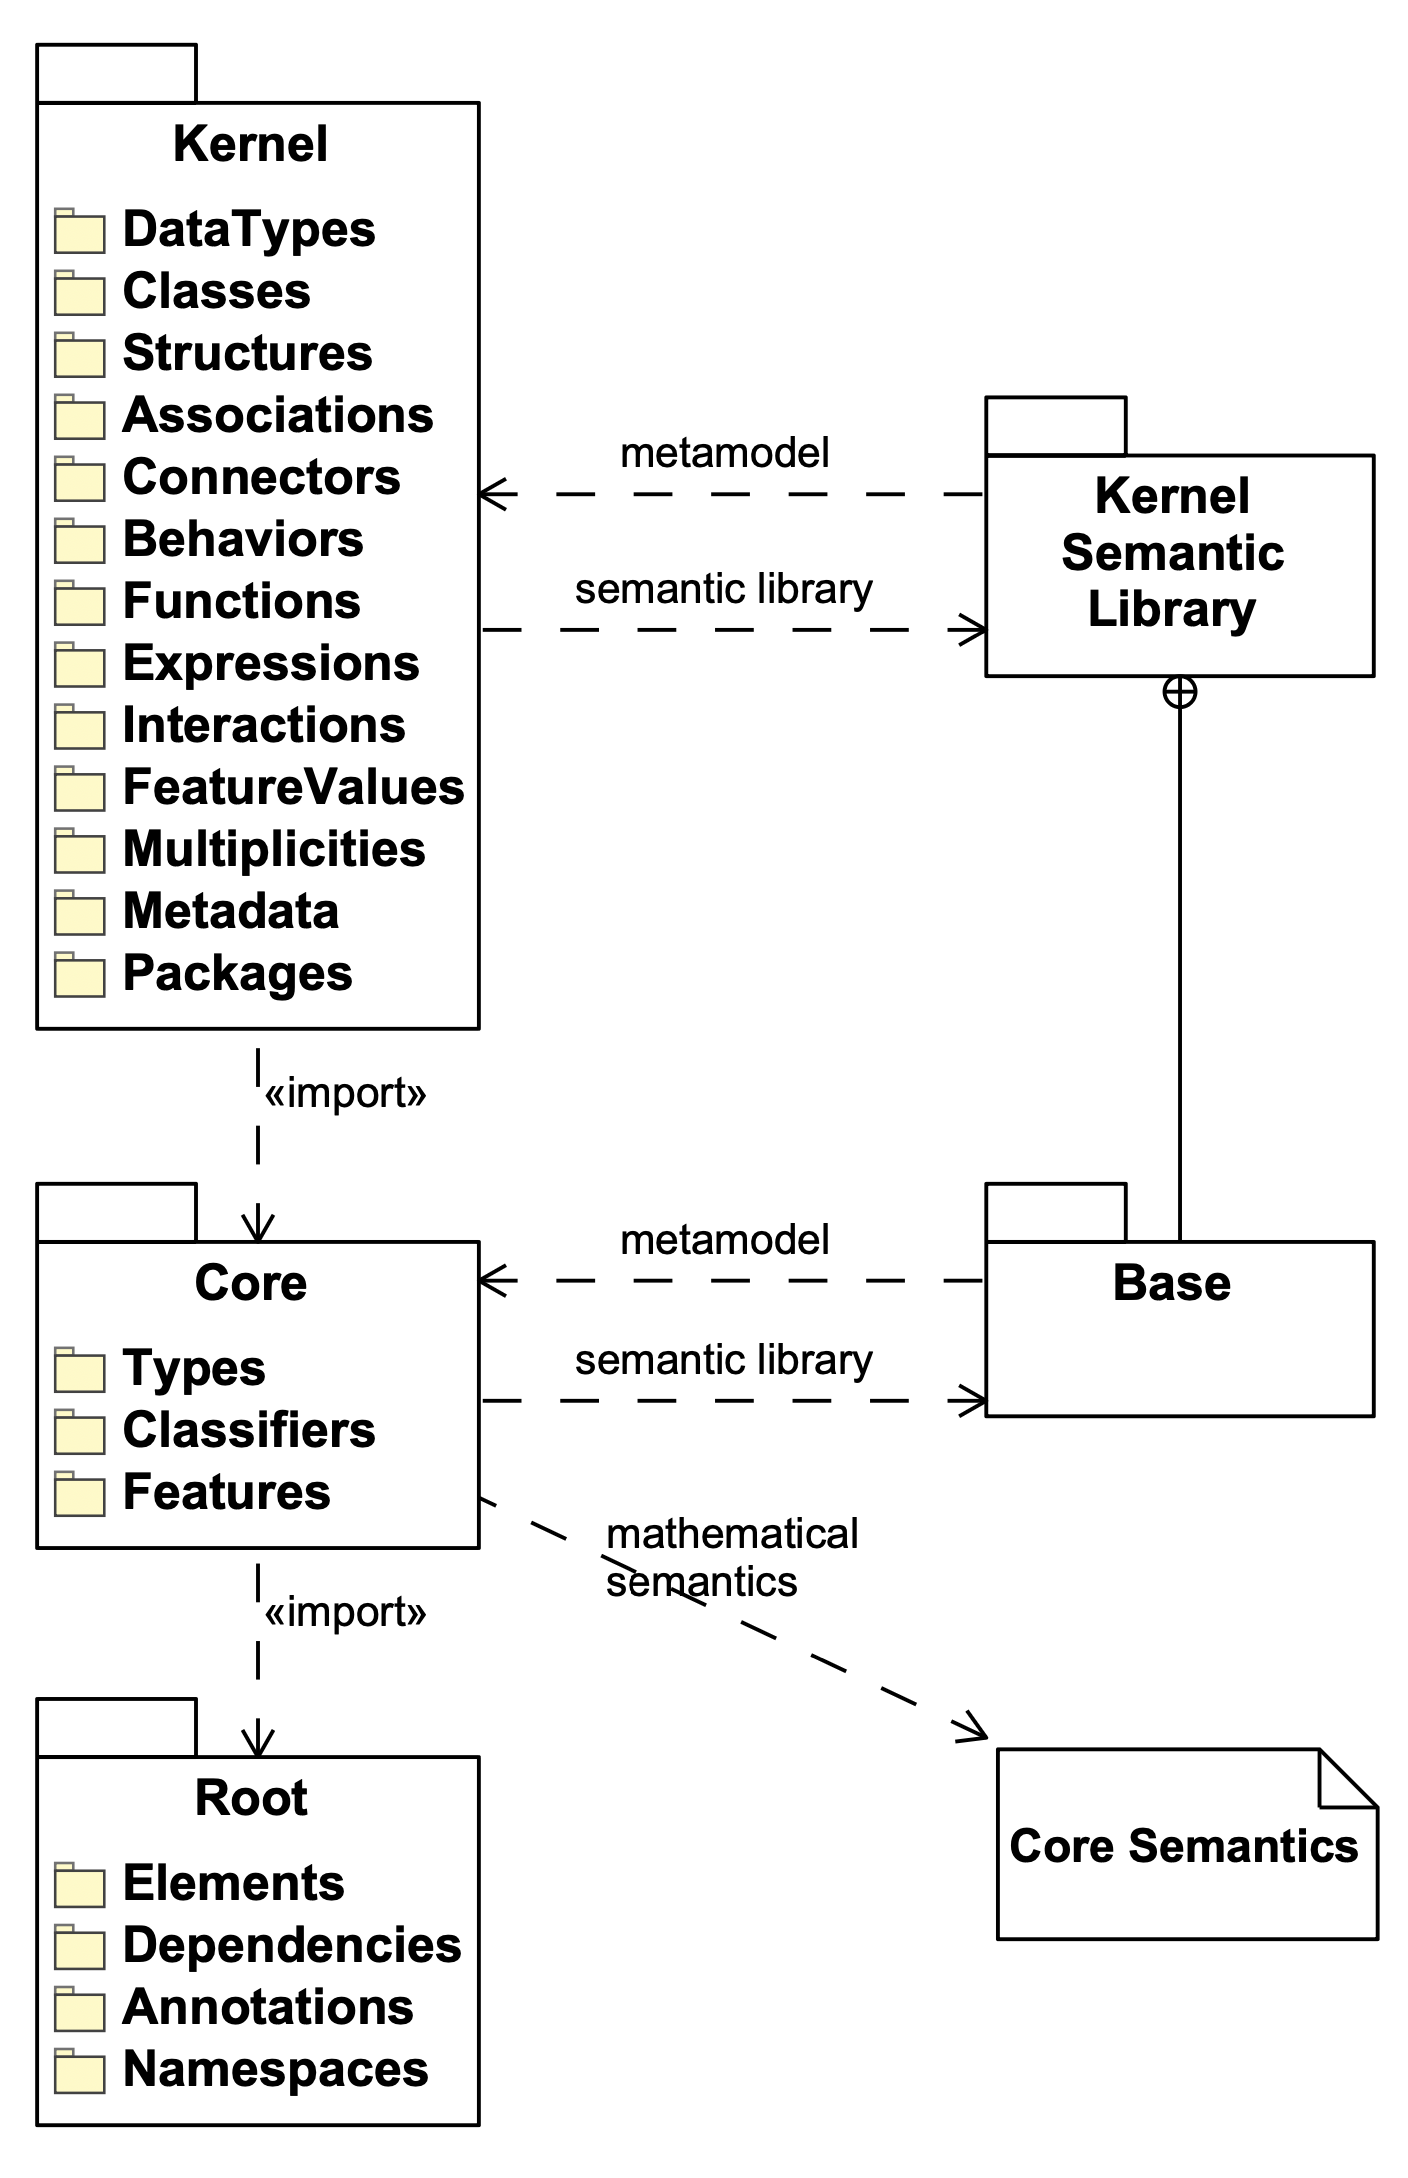
\includegraphics[width=3in]{../pics/Fig41}
\caption{KerML Semantic Layers}
\label{fig:Fig41}
\end{center}
\end{figure}


\pn KerML semantics are specified by a combination of mathematics and model libraries, as illustrated in Figure \ref{fig:Fig41}. The left side of this diagram shows the abstract syntax packages corresponding to the three layers of KerML. The right side shows the corresponding semantic layering.
\begin{enumerate}
\item The Root Layer defines the syntactic foundation KerML and, as such, does not have a semantic interpretation relative to the modeled system.
\item The Core Layer is grounded in mathematical semantics, set theory, supported by the Base package from the Kernel Model Library.  Chapter \ref{chapter:coresemantics} specifies the semantics of the Core layer.
\item The Kernel Layer is also grounded in mathematical semantics, modal logic, particularly for time-varying behavior.
%, supported Model Library  whose static semantics extends the semantic of the Core layer.  
Chapter \ref{chap:kernelsemantics} specifies the semantics of the Kernel layer.
\end{enumerate}

\begin{figure}[htbp]
\begin{center}
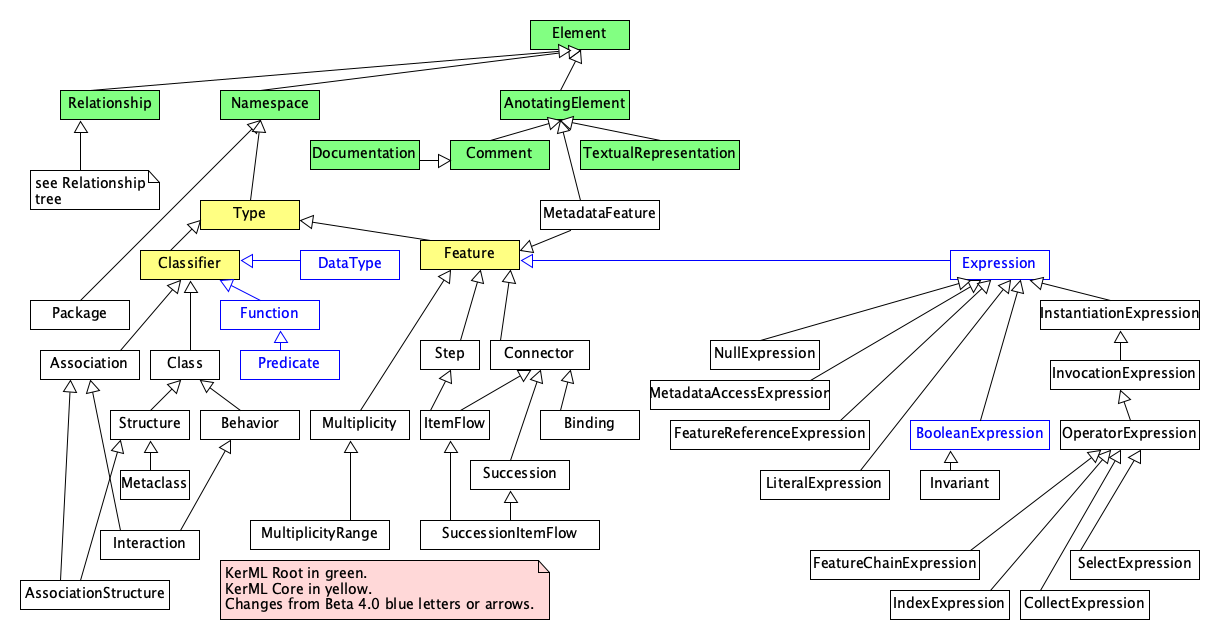
\includegraphics[width=6in]{../pics/KerML-SFS}
\caption{KerML Element Class Diagram}
\label{fig:classdiagram}
\end{center}
\end{figure}

Figure \ref{fig:classdiagram} depicts the class diagram of KerML elements.  By necessity, some subtle yet significant differences are made from KerML \kermlversion.
\begin{description}
\item[DataType ] is a Classifier, disjoint from Class, Function, and Association because a data type is not an element of the system.
%\item[Value ] is an Element, an individual value represented by a set.
\item[Expression ] is a Feature which determines a value.  For calculations performed by the system use \texttt{calc} which is a Behavior, instead.
\item[Function ] is a Classifier which defines a reusable value determination. 
\item[Predicate ] is a Function which defines a boolean value determination.
\item[BooleanExpression ] is a boolean-valued Expression. 
\end{description}

\begin{figure}[htbp]
\begin{center}
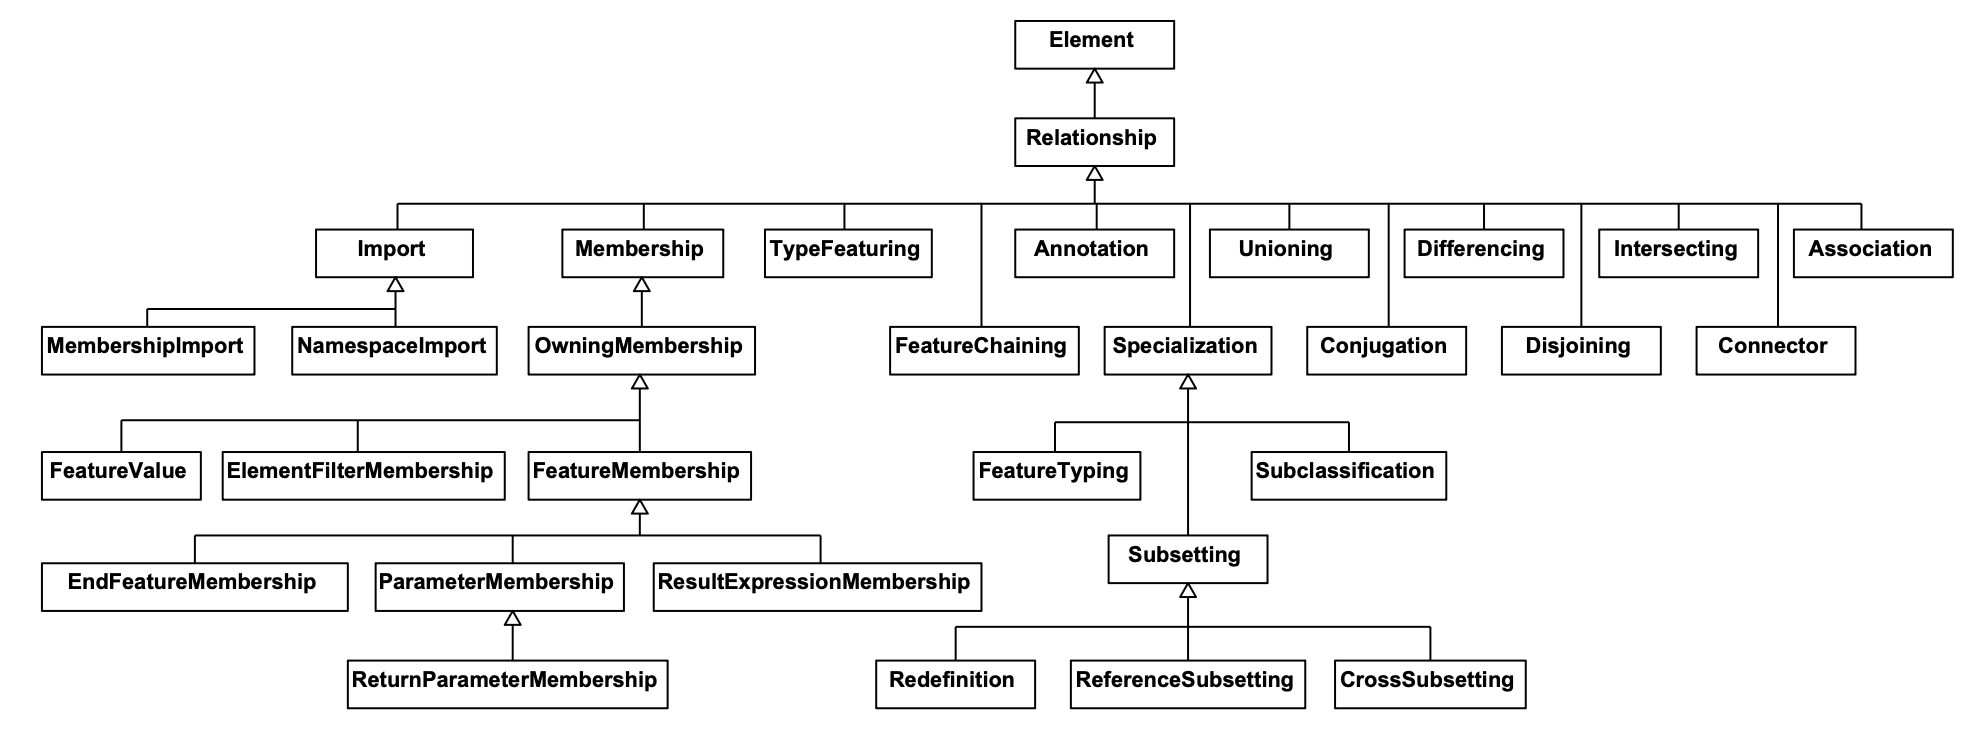
\includegraphics[width=6in]{../pics/relationshipclass}
\caption{KerML Relationship Class Diagram}
\label{fig:relationshipclassdiagram}
\end{center}
\end{figure}

Figure \ref{fig:relationshipclassdiagram} depicts the class diagram of KerML relationships, which are unchanged by SFS.  

\section{Semantic Constraints (KerML 8.4.2)}

\pn KerML semantics are specified by a combination of a mathematical interpretation of the Core
layer, set theory, a mathematical interpretation of the Kernel layer, modal logic, and a set of required relationships between Core and Kernel model elements and elements of the Kernel
Semantic Library (KerML 9.2). The latter relationships are defined by semantic constraints included in the KerML
abstract syntax (see KerML 8.3.1 on the various kinds of constraints in the abstract syntax). Additionally, other
semantic constraints require relationships between elements within a user model necessary for the model to be
semantically well formed.

\pn Specifically, there are four categories of semantic constraints\index{semantic constraint}, each dealing with a different kind of relationship.

\begin{description}
\item[Specialization constraints ] These constraints require that \texttt{Type} elements of a certain kind directly or
indirectly specialize some specific base \texttt{Type} from the Kernel Semantic Library. They are the fundamental
means for providing semantics to abstract syntax elements in the Kernel layer. Specialization constraints
always have the word \texttt{Specialization} in their name.
\item[Redefinition constraints ] These constraints require that certain \texttt{Features} in a model have \texttt{Redefinition} 
relationships with certain other \texttt{Features} in the model. While \texttt{Redefinitions} are kinds of
specializations, redefinition constraints differ from the specialization constraints described above in
that they are between two elements of a user model, rather than between an element of a user model and
an element of a library model. Redefinition constraints always have the word \texttt{Redefinition} in their
name.
\item[Type-featuring constraints ]  These constraints require that certain \texttt{Features} in a model have
 \texttt{TypeFeaturing} relationships with certain other  \texttt{Types} in the model. They arise at points in a model in
which the  \texttt{OwningMembership} structure is different than the required \texttt{Featuring} relationship, so
 \texttt{FeatureMem\-bership} cannot be used. Type-featuring constraints always have the words
 \texttt{TypeFeaturing} in their name.
\item[Binding-connector constraints ]  These constraints require that \texttt{BindingConnectors} exist between certain
\texttt{Features} in a model.
\end{description}

\comment{I am very uncomfortable having tools insert implied relationships to comply with semantic constraints.
I'm sure Ed put some slick helps in the Pilot Implementation so users can leave off `obvious' relationships.
I contend that rather than having tools \emph{may} insert implied \texttt{Relationships}, that those relationships must
always be computable when needed.}






